\chapter{Delayed Measurement and Quantum Eraser}
\section{Introduction}
    The double slit experiment led to discussions about the mysterious quantum mechanics and how to encapsulate the wave nature(the interference behaviour) and particle behaviour(no-interference) of the light into a single unified theory. As per the most common double-slit experiment, either the slit from which the photon passes through is not observed and interference is obtained on the screen or we can place detectors for getting the information about the slit from which the particle is passed and there is no interference. \\ \par
    These two experiments are completely different from each other because we can't detect the slit of the photon without destroying the interference pattern. This is an illustration of the complementarity or the uncertainty principle.
    One of the explanation that can be given is, the observation about the slit causes disturbance to the photon which results to loose the interference pattern. \\ \par
    This led Wheeler to propose ``delayed choice'' experiment to analyze when exactly the photon ``decides'' to which behaviour it is going to adopt. The choice of measurement(whether to measure or not) is made at very last moment.
\section{Delayed Choice Experiment}
\subsection{The experiment:}
    Delayed choice experiment was a an extension of double slit experiment and was proposed by \textbf{Wheeler}, rather than a fixed screen to detect light, it had a removable screen and behind that was two detectors(pointing precisely at each of the slits) for detecting the the slit from which the photons came through. The basic essence of this experiment and the others which followed it, was that the choice to detect the slit from which the photon went through can be made at last moment. If the screen in present we can't get knowledge about the slit from which the photon passed but the interference will be observed, and if the screen is removed then only one of the detector clicks giving us the knowledge about the path of the photon. \\
    \begin{figure}[h]
        \centering
        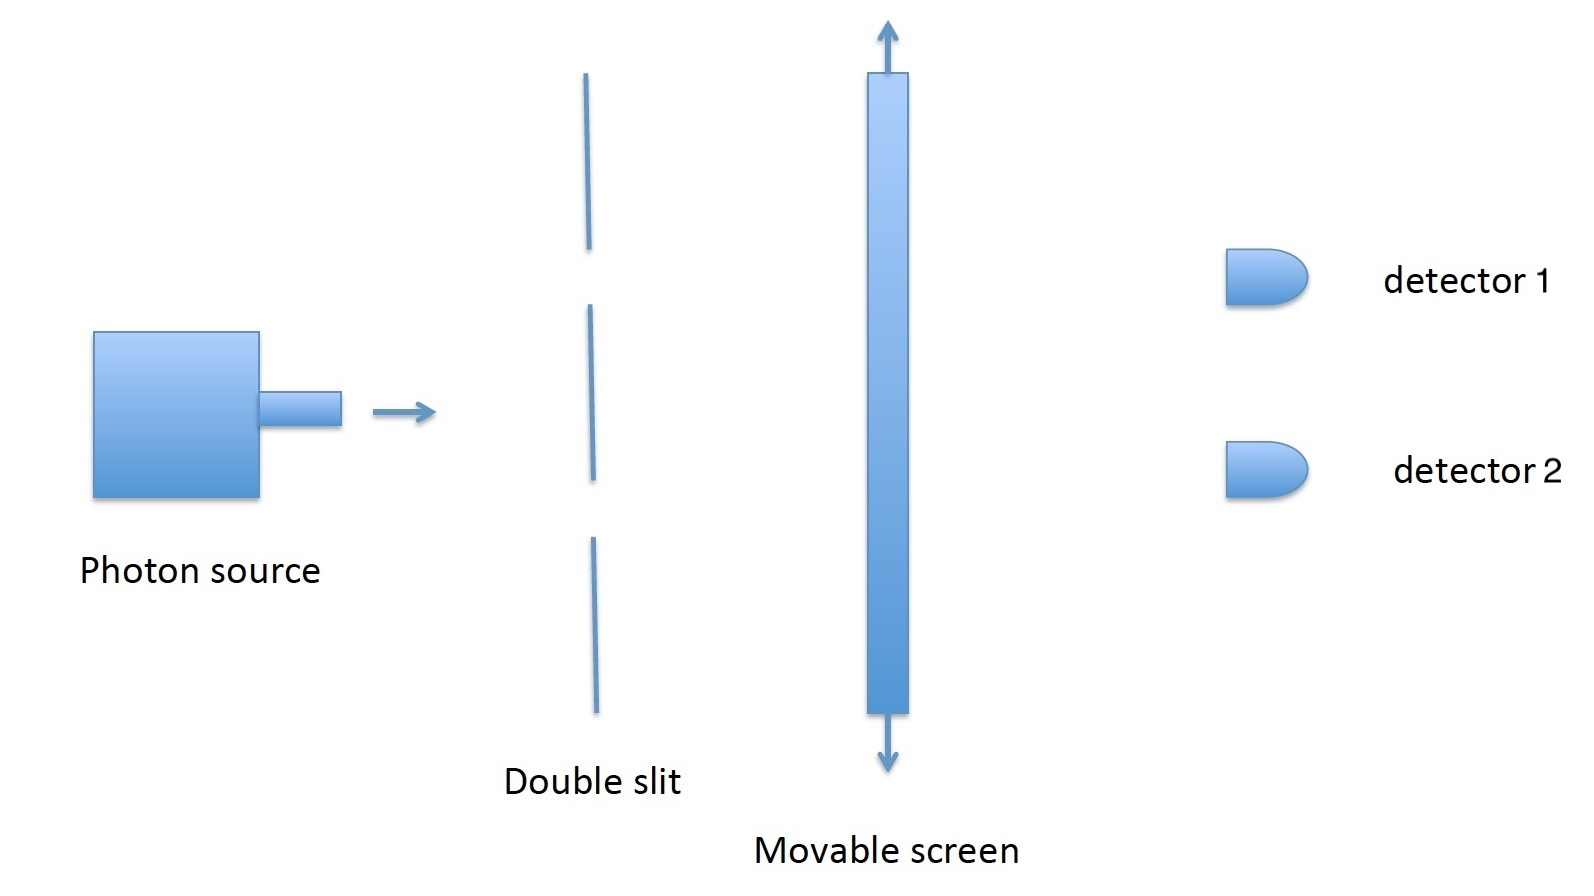
\includegraphics[scale = 0.19]{images/wheeler_delayed.jpg}
        \caption{Delayed choice double slit experiment}
        \label{fig:my_label}
    \end{figure}
    \par The usual presentation of this behaviour can be given as when the screen is present(interference), each photon decides to travel through both of the slits, but when the screen is removed then the photon decides only one of the slit to pass through. \emph{This is strange}. A possible interpretation can be that the photon is ``informed'' of the presence of absence of screen. A delayed choice here means we can increase the distance between the slit and the screen and remove or add the screen well after the time the photon passed through the slit. So in simple but absurd words we can say that ``\emph{the decision to keep or remove the screen is having an influence on the decision that has been made in past}''.
    \subsection{Mathematical Interpretation}
    \subsubsection{When the screen is present}
    We can write the wave function of the photon immediately after it crosses the slits as a sum of two spherical waves:
    \begin{equation}
        \psi(\Vec{r}) = \frac{1}{\lvert \Vec{r} - \Vec{r_1} \rvert}e^{ik\lvert \Vec{r} - \Vec{r_1} \rvert} + \frac{1}{\lvert \Vec{r} - \Vec{r_2} \rvert}e^{ik\lvert \Vec{r} - \Vec{r_2}\rvert}
    \end{equation}
    Where we have k as the wave number of the photon and $\Vec{r_1}$ and $\Vec{r_2}$ are the locations of the slits.
    Also we know the distance between the slits can be approximated to $d \sin \theta$ where d is the distance between the slit and the screen and $\theta$ is the angle between the point of interference and center of the slits. So we can write:
    \begin{equation}
        \lvert \Vec{r} -\Vec{r_1} \rvert - \lvert \Vec{r} -\Vec{r_1} \rvert \sim d\sin \theta
    \end{equation}
    Using this in the expression of the wave function:
    \begin{equation}
        \psi(\Vec{r}) \sim \frac{1}{\lvert \Vec{r} - \Vec{r_1} \rvert}e^{ik\lvert \Vec{r} - \Vec{r_1} \rvert}(1+e^{ikd\sin\theta})
    \end{equation}
    Using this equation we can say that constructive and destructive interference will occur at the points $kd\sin\theta = 2n\pi$ and $kd\sin\theta = 2(n+1)\pi$ respectively. Thus the light will be showing a wave like behaviour and the screen is behaving as an apparatus that measures continuous position variable.
    \subsubsection{When the screen is absent}
    Now if we remove the screen and the measure the momentum(detectors measure the momentum of the incoming photons) the incoming photons with a narrow detection range then we can write the wave function as:
    \begin{equation}
        \psi(\Vec{r}) \sim \frac{1}{\lvert \Vec{r} - \Vec{r_1} \rvert}e^{i\Vec{k_1}(\Vec{r} - \Vec{r_1})} + \frac{1}{\lvert \Vec{r} - \Vec{r_2} \rvert}e^{i\Vec{k_2}(\Vec{r} - \Vec{r_2})}
    \end{equation}
    Where $\Vec{k_1}$ and $\Vec{k_2}$ are wave-vectors of size $k$ in the direction of slit to the point of detection, direction specifically given by $\Vec{r_T} - \Vec{r_1}$ and $\Vec{r_T} - \Vec{r_2}$ where $\Vec{r_T}$ is the location of the detectors(since we are considering narrow detection range).\\
    \par Since the detector measures the momentum of the incoming photon we can say that when the detector1($D_1$) clicks, the momentum of photon becomes close to $\Vec{k_1}$ and when detector2($D_2$) clicks, the momentum of photon becomes close to $\Vec{k_2}$. We can consider this as an apparatus that measures a two valued($D_1$ and $D_2$) momentum observable. So when the wavefunction is measured using this apparatus, it can be written as:
    \begin{equation}
        \psi(\Vec{r}) \sim \frac{1}{\lvert \Vec{r} - \Vec{r_1} \rvert}e^{i\Vec{k_1}(\Vec{r} - \Vec{r_1})} \ket{D_1 clicks} + \frac{1}{\lvert \Vec{r} - \Vec{r_2} \rvert}e^{i\Vec{k_2}(\Vec{r} - \Vec{r_1})} \ket{D_2 clicks}
    \end{equation}
    (Wavefunction not normalised) \\
    Thus we have a superposition of states and the probability of each of the states $D_1$ and $D_2$ click are proportional to $\frac{1}{\lvert \Vec{r} - \Vec{r_1} \rvert}$ and $\frac{1}{\lvert \Vec{r} - \Vec{r_2} \rvert}$ respectively, which are equal, so clicking of each detector has a 50 percent probability.
    \subsection{Possible Explanation}
    The mathematical formulation gives us an idea about how the weird behaviour of the delayed measurement can be explained, the argument that the path followed by the photon is dependent on its measurement is false. A better explanation to this will be that the photon has quantum behaviour(as depicted by $\psi(\Vec{r})$in equation 1) from the moment it is generated till point it is measured(by the screen or the detector), that is until a measurement is made on it. \\
    \par It means that photon as depicted by $\psi(\Vec{r})$ follows both the route until it is measured. After the measurement, the quantum state(wave function) collapses to one of the possible eigen-vector of the observable measured(two valued momentum observable in case of the detectors and a continuous position observable in case of screen). This measurement is reflected by the interference pattern on the screen or the clicking of the detector in their respective experiment setup.\\ 
    \par Considering all the counter arguments against the claim, ``that you can influence the decisions of the past'', it now seems useless because the photon followed both the path before it was measured and removing or adding the screen at the very last moment seems of no special interest now.
    \section{Delayed Choice Quantum Erasure}
    These experiments are somewhat a generalisation of the entanglement situation. They show that the loss of interference or information about the slit on one particle is not due to the uncertainty principle, but because of the measurement of the twin(entangled) particle.
    \begin{figure}[ht]
        \centering
        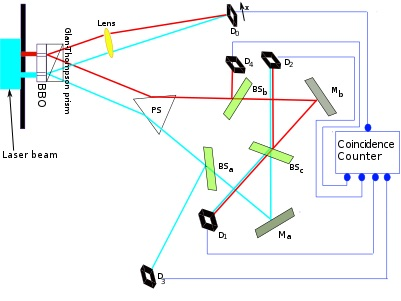
\includegraphics[scale = 0.7]{images/quantum_eraser.jpg}
        \caption{Delayed choice quantum eraser}
        \label{fig:my_label}
    \end{figure}
    \subsection{Experiment}
    For this experiment after the point when the photons passes through the slits, they are encountered by BBO crystal, which converts each of the photon into two entangled photons of half energy than the original photon, here $D_0$ is a movable detector that detects the interference pattern for the photons that are travelling upward(called the \emph{signal photons}) and the photons travelling downwards(called the \emph{idler photons}) are received by a prism and a set of beam splitters(BS) and mirrors(M). The idler photons then are detected by the detectors $D_1 - D_4$(depending upon the path the photon chooses). Also the setup is such that path of signal photons from the crystal to the detector is shorter as compared to the path in case of idler photons. \\
    \par Here we can see that if the detectors $D_3$ or $D_4$ clicks then the photon has travelled through one of the routes, but if the detectors $D_1$ or $D_2$ clicks then we are not sure about the path that the photon has travelled. The beam splitter $BS_c$ is acting as a quantum erasure because if it present it no more possible to know the path of the photon which was detected by $D_1$ and $D_2$ and if it is absent then we can know the path of the photons, if $D_1$ clicks then upper slit and if $D_2$ clicks then the lower slit and the interference pattern is lost. \\
    \par So we can say that the keeping or removing of the quantum eraser is affecting the measurement of the signal photons, but the measurement of the signal photons is done earlier in time(because of short path). \emph{This is quite strange}. Another argument to this can be that the measurement and the results of the detector 0 can be used to predict the future(whether the quantum eraser is removed in future or not). \emph{Again this is also quite strange}.
    \subsection{Discussion}
    At first glance at the observations of the experiment seems very amusing but they are quite misleading. One important point to notice here is that, it is possible to extract an interference pattern or a discrete pattern only through extraction from all the detections by $D_0$ for corresponding $D_i 's$. Blatantly looking for pattern at $D_0$ doesn't gives us anything but a pattern of random points. Mathematically we can say that
    \begin{equation*}
        D_0 = \sum_{i=1}^{4}D_i
    \end{equation*}
    Meaning that the information(peak and troughs) at $D_0$ is the sum of the information of all sensors, detected using the idler photos. \\
    \par This has a consequence, that it is impossible to use this device to transmit information from the future to the past because recognizing an interference pattern is possible only when one have the knowledge of which detection of signal photon by $D_0$ corresponds to which detector $D_i$ of the twin idler photon. \\
    \par The tempting idea of removing or adding the beam splitter($BS_0$) in far future to produce the interference($BS_0$ present) or to remove the interference($BS_0$ absent) in present, is not working because of the fact that you can't extract the information about the interference patter of discrete pattern just by looking at the screen(detector $D_0$), since the interference pattern related to $D_1$ and $D_2$ have a $\pi$ phase shift, thus they produce exactly the same image as it is produced when there is no interference pattern.
    \subsection{Mathematical Interpretation}
    We can use the fact about the entangled particles that the order of measurement does not affect the conditional probabilities. \\
    We can write the wave function right after the slit but before the crystal as:
    \begin{equation}
        \ket{I} \xrightarrow[]{} \frac{1}{\sqrt{2}}[\ket{U}+\ket{L}]
    \end{equation}
    Where $\ket{U}$ and $\ket{L}$ signifies photons passing through upper slit and lower slit respectively, equation 6 signifies the superposition of the paths. Then the each component are split into entangled pairs, one going upwards and one going downwards.
    \begin{equation}
        \ket{\psi} \xrightarrow{} \frac{1}{\sqrt{2}}\left[\ket{US}\ket{UI} + \ket{LS}\ket{LI}\right]
    \end{equation}
    Where S and I indicates the signal and idler photons(for example $\ket{US}$ refers to photon coming from upper slit and going upward towards the screen $D_0$). \\
    Now the idler photons are measured by the set of detectors $D_1 - D_4$, we can mathematically write this as:
    \begin{equation}
        \ket{]\psi} \xrightarrow[]{} \ket{US}\left[\frac{1}{2}\ket{4} + \frac{1}{2\sqrt{2}}\ket{1} + \frac{1}{2\sqrt{2}}\ket{2}\right] + \ket{LS} \left[\frac{1}{2}\ket{3} + \frac{1}{2\sqrt{2}}\ket{1} + \frac{1}{2\sqrt{2}}\ket{2} \right]
    \end{equation}
    This equation is similar to equation of bell's entangled pair(EPR pair), to see it more clearly we can write it as:
    \begin{equation}
        \ket{]\psi} \xrightarrow[]{} \ket{U}^S\left[\frac{1}{2}\ket{4} + \frac{1}{2\sqrt{2}}\ket{1} + \frac{1}{2\sqrt{2}}\ket{2}\right]^I + \ket{L}^S \left[\frac{1}{2}\ket{3} + \frac{1}{2\sqrt{2}}\ket{1} + \frac{1}{2\sqrt{2}}\ket{2} \right]^I
    \end{equation}
    Wave function for an entangled pair can be written as:
    \begin{equation}
        \ket{\psi} = \frac{1}{\sqrt{2}}\left[\ket{+}^A\ket{-}^B - \ket{-}^A\ket{+}^B\right]
    \end{equation}
    Here S and I stands for two entangled particles A and B, and $\ket{U}$ and $\ket{L}$ stands for the states of particle A $\ket{+}$ and $\ket{-}$, while the second part of both terms stand respectively for states $\ket{-}$ and $\ket{+}$ for particle B.
    So we can see that equation 9 and 10 are similar and equation 10 represent entangled particles. \\
    Now we know that the correlations between the measurements on the two particles will be independent of the order in which the measurements are done. So we can assume that the measurement of the idler photon is done first. We can rewrite the equation 9 as:
    \begin{equation}
        \ket{\psi} = \frac{1}{2\sqrt{2}}\ket{1}^I \left[\ket{U} + \ket{L}\right]^S + \frac{1}{2\sqrt{2}}\ket{2}^I \left[\ket{U} + \ket{L}\right]^S + \frac{1}{2}\ket{4}^I\ket{U}^S
    \end{equation}
    Now if we look at the wave function written in this form we can see that when the idler photon is detected by $D_1$ or $D_2$ then we will observe an interference pattern for the signal photon and the path of the photon will be unknown and if it is detected by $D_3$ or $D_4$ then we will not have interference pattern for the signal photon but will have deterministic knowledge about the slit from which the photon came through.
    \begin{itemize}
        \item While this mathematical interpretation may seem clear because we reversed the order of measurement arguing the independence of order of measurement on entangled particles, but the very physical meaning of this order independence is quite unclear.
        \item Another problem is that we are taking for granted the reduction postulate and the collapse of the wave function.
    \end{itemize}
    \section{Conclusion}
    Thus the reasoning of this experiment came to the phenomena of entanglement and how it can happen in time independent manner and what is the physical meaning of collapse of wave function. These are one of the most weird and controversial results of the quantum mechanics. \\
    \par But thinking from a different view, we can use this experiment to understand how a quantum mechanics system hides information from us, we tried our best to get the path as well the interference pattern for the photon but the quantum mechanical system chose to hide it from us. \\
    \par This can be pointed out as one of the short comings of quantum information and quantum computation(because if it is possible then you can get exponential increase on already existing quantum computing algorithms which are themselves a big improvement on the classical algorithms), you can be so close to the solution but still be very far, because of the very reason that you can't access the probability distribution of a single particle, because as soon as you measure it, the wave function collapse.
